\documentclass[12pt]{article} 
\usepackage[utf8]{inputenc} 
\usepackage[english]{babel} 
\usepackage{amsmath, amssymb, amsthm, bm} 
\usepackage{geometry} 
\usepackage{tikz} 
\usetikzlibrary{shapes, backgrounds, decorations.pathreplacing, positioning, arrows.meta, calc, fit} 
\usepackage{caption} 
\usepackage{setspace} 
\usepackage{enumitem} 
\usepackage{booktabs} 
%\usepackage[backend=biber,style=chicago-authordate]{biblatex}
\usepackage[round]{natbib}

% Hyperref for clickable Table of Contents and citations 
\usepackage{hyperref} 
\hypersetup{ 
	colorlinks=true, 
	linkcolor=blue, 
	filecolor=magenta,
	urlcolor=cyan, 
	citecolor=red, 
}

% Custom theorem styles 
\newtheorem{theorem}{Theorem}[section] 
\newtheorem{lemma}[theorem]{Lemma} 
\newtheorem{definition}{Definition}[section] 
\newtheorem{example}{Example}[section] 
\newtheorem{proposition}{Proposition}[section]

\geometry{letterpaper, margin=1in} 
\onehalfspacing

\begin{document}
	
	\title{A Non-Compact Formulation and Complexity Framework for the Tool Switching Problem}
	\author{Shankar Narayanan \\
		\textit{Internship Report} \\
		Advisors: Prof. Rafael Colares and Prof. Annegret Wagler}
	\date{March 30, 2026}
	\maketitle
	
	\begin{abstract}
		The management of tool configurations in Flexible Manufacturing Systems (FMS) is a well-studied NP-hard combinatorial optimization challenge. This report provides a mathematical analysis of the sequential Tool Switching Problem (SSP) by evaluating its non-compact formulation. We systematically establish the structural equivalences of the SSP to classical optimization frameworks, specifically mapping its continuous routing to the Generalized Traveling Salesman Problem (GTSP) and its configuration bounds to the Job Grouping Problem (JGP). Furthermore, we establish a strict distinction between the Uniform SSP (U-SSP) and the Tool-Dependent SSP (TD-SSP), proving that the JGP serves as the exact operational objective for the latter via Lexicographical Minimization. Finally, we demonstrate that the dynamic generation of these configurations within an exact Branch-and-Price framework is mathematically equivalent to the Set Union Knapsack Problem (SUKP), explicitly necessitating Machine Learning interventions to accelerate the NP-hard pricing oracle.
	\end{abstract}
	
	\section{Introduction}
	
	Flexible Manufacturing Systems (FMS) enable rapid adaptation to market changes by utilizing numerically controlled machines equipped with automated tool magazines. Because a single machine may be required to process a diverse batch of parts, and because the total number of distinct tools required often exceeds the capacity of the machine's magazine, tool switches are unavoidable \citep{Tang1988}. A tool switch incurs a time penalty that delays production. Consequently, optimal tool management is a primary objective in manufacturing optimization.
	
	This report focuses on the Job Sequencing and Tool Switching Problem (SSP). In this problem, a set of jobs must be processed on a single machine equipped with a tool magazine of limited capacity. Each job requires a specific subset of tools, and all required tools must be present in the magazine before the job can be processed. The objective is to determine a processing sequence for the jobs and an associated tool loading policy that jointly minimize the total cost or number of tool switches.
	
	Because the SSP is strongly NP-hard \citep{Crama1994}, modern solution methodologies rely on decomposition. As formally proven by \citet{Tang1988}, the SSP naturally decomposes into two nested subproblems: the \textbf{Sequencing Problem (SP)} (determining the optimal job order) and the \textbf{Tooling Problem (TP)} (determining the optimal tool loading and eviction policy for a fixed sequence).
	
	To accurately model the computational complexity of the TP, the literature strictly distinguishes between two variants of the problem, which we will formally define and utilize throughout this report:
	\begin{itemize}[noitemsep]
		\item \textbf{Uniform SSP (U-SSP):} The standard variant where the time or effort required to change any tool is identical (a uniform cost of 1). The objective is to minimize the absolute \textit{number} of individual tool switches.
		\item \textbf{Tool-Dependent SSP (TD-SSP):} A complex real-world variant where setup times are non-uniform and vary significantly depending on the specific tool being inserted or removed. 
	\end{itemize}
	
	To develop a state-of-the-art exact solver, it is imperative to move beyond isolated heuristics and situate the SSP within the broader landscape of Combinatorial Optimization (CO). The primary objective of this report is to analyze the non-compact formulation of the SSP by proving its mathematical equivalence to other classical CO domains, thereby justifying an advanced algorithmic architecture.
	
	The remainder of this report is structured as follows. Section 2 introduces the non-compact mathematical formulation, scoped strictly to the U-SSP. Section 3 maps the continuous routing state space of the U-SSP to the Generalized Traveling Salesman Problem (GTSP). Section 4 analyzes the configuration bounds provided by the Job Grouping Problem (JGP), and resolves the operational differences between the U-SSP and TD-SSP via Lexicographical Minimization. Section 5 formalizes the exact Branch-and-Price pricing oracle as the Set Union Knapsack Problem (SUKP). Finally, Sections 6 and 7 outline cutting-edge Machine Learning pathways—such as Neural Column Generation—designed to bypass this NP-hard pricing bottleneck.

	
	
	\section{The Non-Compact Formulation for the U-SSP}
	\label{sec:non_compact}
	
	In order to solve the Uniform SSP exactly, we must first map its state space. Traditionally, compact Integer Linear Programming (ILP) formulations attempt to model the exact placement of individual tools in the magazine slots at each discrete time step. However, to overcome the severe symmetry issues inherent in those compact models, state-of-the-art approaches utilize a non-compact formulation based on routing between maximal tool configurations.
	
	\textbf{Scope of Analysis:} Throughout Section \ref{sec:non_compact}, Section 3, and Sections 4.1--4.3, we operate strictly under the \textbf{Uniform SSP (U-SSP)} assumption. This means that the time or effort required to insert or remove any individual tool is identical. This assumption is mathematically critical because it guarantees that the cost of transitioning between any two states of the machine is symmetric and exactly proportional to the discrete number of exchanged tools.
	
	The computational complexity of the SSP is fundamentally rooted in its state space. Traditional compact models sequence the jobs directly and track tool insertions step-by-step. However, these models suffer from symmetry caused by 0-blocks. As formally defined by \citet{Crama1994}, a 0-block is a maximal subset of consecutive zeros in a row of the tool-job incidence matrix—representing a time interval before and after which a tool is needed, but during which it is not required.
	
	The act of retaining an unneeded tool in the magazine across this gap to avoid redundant unloading and reloading is mathematically referred to as ``flipping'' the 0-block to 1s. This structure forces compact solvers to evaluate highly symmetric, redundant permutations to decide which 0-blocks to flip, severely limiting computational performance \citep{Catanzaro2015}.
	
	\subsection{Illustrative Example: Magazine State Evolution}
	
	To illustrate the tool switching mechanics and the concrete impact of flipping a 0-block, consider the 5-job, 7-tool instance. The machine has a magazine capacity of $b = 4$, and the jobs are processed in the sequence $j_1 \to j_2 \to j_3 \to j_4 \to j_5$. The specific tool requirements for each job are illustrated in the incidence matrix in Figure \ref{fig:incidence_matrix}.
	
	\begin{figure}[h!]
		\centering
		$
		\begin{array}{c|ccccc}
			& j_1 & j_2 & j_3 & j_4 & j_5 \\
			\hline
			t_1 & 1 & 0 & 0 & 1 & 1 \\
			t_2 & 1 & 1 & 0 & 0 & 1 \\
			t_3 & 1 & 1 & 0 & 0 & 0 \\
			t_4 & 0 & 1 & 1 & 0 & 0 \\
			t_5 & 0 & 0 & 1 & 1 & 0 \\
			t_6 & 0 & 0 & 1 & 1 & 0 \\
			t_7 & 0 & 0 & 0 & 0 & 1 \\
		\end{array}
		$
		\caption{An incidence matrix for a 5-job, 7-tool instance. The machine magazine has a capacity $b=4$. Assuming the sequence $j_1 \to j_2 \to j_3 \to j_4 \to j_5$, tool $t_1$ is required by jobs $j_1, j_4$, and $j_5$, but not by $j_2$ and $j_3$. This gap of non-requirement represents a 0-block for $t_1$. Because $b=4$ is large enough to accommodate the transition tool requirements, the optimal policy evaluates whether to ``flip'' this 0-block by retaining $t_1$ through jobs $j_2$ and $j_3$ to avoid redundant setups.}
		\label{fig:incidence_matrix}
	\end{figure}
	
	The specific tool requirements for each job are as follows:
	\begin{itemize}[noitemsep]
		\item $T_1 = \{t_1, t_2, t_3\}$
		\item $T_2 = \{t_2, t_3, t_4\}$
		\item $T_3 = \{t_4, t_5, t_6\}$
		\item $T_4 = \{t_1, t_5, t_6\}$
		\item $T_5 = \{t_1, t_2, t_7\}$
	\end{itemize}
	
	Under the optimal Keep Tool Needed Soonest (KTNS) policy \citep{Tang1988}, the solver looks ahead to determine which 0-blocks to flip to minimize future swaps. The evolution of the optimal magazine configurations across this sequence is depicted in Figure \ref{fig:magazine_evolution}.
	
	\begin{figure}[h!]
		\centering
		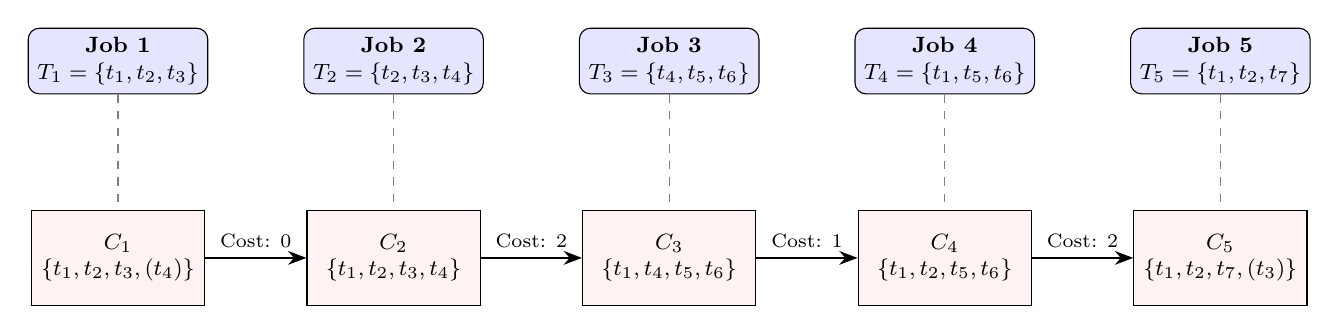
\begin{tikzpicture}[
			jobnode/.style={draw, rectangle, rounded corners, fill=blue!10, minimum width=2.2cm, minimum height=0.8cm, align=center, font=\footnotesize\bfseries},
			magnode/.style={draw, rectangle, fill=red!5, minimum width=2.2cm, minimum height=1.2cm, align=center, font=\footnotesize},
			arrow/.style={-Stealth, thick}
			]
			% Jobs
			\node[jobnode] (j1) at (0, 2.5) {Job 1 \\ $T_1=\{t_1, t_2, t_3\}$};
			\node[jobnode] (j2) at (3.5, 2.5) {Job 2 \\ $T_2=\{t_2, t_3, t_4\}$};
			\node[jobnode] (j3) at (7, 2.5) {Job 3 \\ $T_3=\{t_4, t_5, t_6\}$};
			\node[jobnode] (j4) at (10.5, 2.5) {Job 4 \\ $T_4=\{t_1, t_5, t_6\}$};
			\node[jobnode] (j5) at (14, 2.5) {Job 5 \\ $T_5=\{t_1, t_2, t_7\}$};
			
			% Magazines
			\node[magnode] (m1) at (0, 0) {$C_1$ \\ $\{t_1, t_2, t_3, (t_4)\}$};
			\node[magnode] (m2) at (3.5, 0) {$C_2$ \\ $\{t_1, t_2, t_3, t_4\}$};
			\node[magnode] (m3) at (7, 0) {$C_3$ \\ $\{t_1, t_4, t_5, t_6\}$};
			\node[magnode] (m4) at (10.5, 0) {$C_4$ \\ $\{t_1, t_2, t_5, t_6\}$};
			\node[magnode] (m5) at (14, 0) {$C_5$ \\ $\{t_1, t_2, t_7, (t_3)\}$};
			
			% Arrows
			\draw[arrow] (m1) -- (m2) node[midway, above, font=\scriptsize] {Cost: 0};
			\draw[arrow] (m2) -- (m3) node[midway, above, font=\scriptsize] {Cost: 2};
			\draw[arrow] (m3) -- (m4) node[midway, above, font=\scriptsize] {Cost: 1};
			\draw[arrow] (m4) -- (m5) node[midway, above, font=\scriptsize] {Cost: 2};
			
			% Vertical links
			\draw[dashed, gray] (j1) -- (m1);
			\draw[dashed, gray] (j2) -- (m2);
			\draw[dashed, gray] (j3) -- (m3);
			\draw[dashed, gray] (j4) -- (m4);
			\draw[dashed, gray] (j5) -- (m5);
		\end{tikzpicture}
		\caption{Evolution of the optimal magazine configurations across the job sequence with capacity $b=4$. Notice how tool $t_1$ is retained in configurations $C_2$ and $C_3$ despite not being required, successfully flipping the 0-block to save future tool switches.}
		\label{fig:magazine_evolution}
	\end{figure}
	
	To bypass the sequence-based symmetry inherent in determining which 0-blocks to flip step-by-step, we utilize the non-compact formulation proposed by \citet{Colares2026}, which projects the problem entirely onto a complete directed graph of valid configurations.
	
	\subsection{Definitions, Variables, and Maximal Configurations}
	
	Let $J = \{1, 2, \dots, n\}$ be the set of jobs and $T = \{1, 2, \dots, m\}$ be the set of all available tools. Each job $j \in J$ requires a specific subset of tools $T_j \subseteq T$. The machine's tool magazine has a capacity $b$.
	
	A fundamental property of this formulation is the assumption of maximal configurations. Let $\mathcal{C} = \{C \subseteq T \mid |C| \le b\}$ be the collection of all valid tool configurations. Without loss of generality, we establish that the tool repository is always full, i.e., $|C| = b$ for all considered configurations \citep{Colares2026}.
	
	\begin{proposition}[Configuration Maximization]
		Any configuration $C$ where $|C| < b$ is strictly dominated by a maximal configuration $C' = C \cup T_{dummy}$ where $|C'| = b$.
	\end{proposition}
	\begin{proof}
		Let $d(C_1, C_2)$ be the number of tool switches required to transition from configuration $C_1$ to $C_2$. Under the U-SSP assumption, the cost formula evaluates to $d(C_1, C_2) = b - |C_1 \cap C_2|$. If $|C_1| < b$, the empty slots can be filled with arbitrary tools from $T \setminus C_1$ to form $C'_1$, yielding $|C'_1| = b$. Because $C_1 \subseteq C'_1$, it mathematically follows that $|C_1 \cap C_2| \le |C'_1 \cap C_2|$. Therefore, $b - |C'_1 \cap C_2| \le b - |C_1 \cap C_2|$. Padding an under-capacity configuration incurs a mathematical penalty of zero while strictly increasing the probability that the added tools may satisfy subsequent job requirements.
	\end{proof}
	
	Let $H_j \subseteq \mathcal{C}$ denote the subset (cluster) of configurations that are capable of processing job $j \in J$. That is, $H_j = \{C \in \mathcal{C} \mid T_j \subseteq C\}$. The U-SSP can now be seen as finding the shortest sequence of configurations in a complete directed graph $K_p$, where $V(K_p) = \mathcal{C}$, visiting at least one vertex from each cluster $H_j$.
	
	Let $y(v)$ denote a binary variable stating whether or not configuration $v \in V(K_p)$ is used to carry some job. Let $x(u, v)$ denote a binary variable stating whether or not configuration $v \in V(K_p)$ is applied right after configuration $u \in V(K_p)$. The U-SSP can thus be modeled as follows:
	
\begin{align}
	\min \quad & \sum_{u \in V} \sum_{v \in V} d(u, v) x(u, v) \label{eq:obj} \\
	\text{subject to} \quad & \sum_{v \in H_j} y(v) \ge 1, \quad \forall j \in J \label{eq:cover} \\
	& \sum_{u \in V} x(u, v) = y(v), \quad \forall v \in V \label{eq:flow_in} \\
	& \sum_{u \in V} x(v, u) = y(v), \quad \forall v \in V \label{eq:flow_out} \\
	& \sum_{u \in H(S)} \sum_{v \in H(S)} x(u, v) \le \sum_{v \in H(S)} y(v) - 1, \quad \forall S \subseteq J, 2 \le |S| \le |J| - 1 \label{eq:gsec} \\
	& x(u, v) \in \{0,1\}, \quad \forall u, v \in V \label{eq:domain_x} \\
	& y(v) \in \{0,1\}, \quad \forall v \in V \label{eq:domain_y}
\end{align}
where $H(S) = \bigcup_{j \in S} H_j$.

To establish the correctness of this formulation, we must prove that the constraints mathematically enforce a valid, continuous sequence of configurations that covers all jobs, and that the objective evaluates the optimal tool switching cost without loss of generality.

\begin{lemma}[Flow and Cover Feasibility]
	Constraints (\ref{eq:flow_in}), (\ref{eq:flow_out}), and (\ref{eq:gsec}) ensure that the selected configurations form a valid, continuous routing sequence without disconnected sub-cycles.
\end{lemma}
\begin{proof}
	Constraints (\ref{eq:flow_in}) and (\ref{eq:flow_out}) enforce strict flow conservation for any selected configuration ($y(v) = 1$). Constraint (\ref{eq:gsec}) operates as the Generalized Subtour Elimination Constraint (GSEC). For any proper subset of jobs $S$, the number of internal transitions within the configurations covering $S$ cannot exceed the total number of configurations covering $S$ minus 1, strictly preventing closed sub-cycles disjoint from the main tour.
\end{proof}

\begin{lemma}[Subtour Elimination]
	Constraint (\ref{eq:gsec}) guarantees that the active configurations form exactly one connected Hamiltonian cycle.
\end{lemma}
\begin{proof}
	Suppose, for the sake of contradiction, that a feasible solution satisfying (\ref{eq:cover})--(\ref{eq:gsec}) forms $k \ge 2$ disjoint directed cycles, $W_1, W_2, \dots, W_k$. Let $V(W_1)$ be the set of active vertices in cycle $W_1$. Let $S \subset J$ be the proper subset of jobs covered exclusively by the configurations in $W_1$. Because $k \ge 2$ and the clusters $H_j$ partition the job requirements, $W_1$ cannot process all jobs without rendering the other cycles completely redundant. Thus, $2 \le |S| \le |J| - 1$.
	
	By definition, all vertices in $W_1$ belong to $H(S) = \bigcup_{j \in S} H_j$, meaning $V(W_1) \subseteq H(S)$. If we sum the selected edges $x(u, v)$ within $W_1$, we have:
	\begin{equation}
		\sum_{u \in V(W_1)} \sum_{v \in V(W_1)} x(u, v) = |V(W_1)| = \sum_{v \in V(W_1)} y(v)
	\end{equation}
	
	Since $V(W_1) \subseteq H(S)$, evaluating the Subtour Elimination Constraint (\ref{eq:gsec}) strictly over $S$ yields:
	\begin{equation}
		\sum_{u \in H(S)} \sum_{v \in H(S)} x(u, v) \ge \sum_{v \in V(W_1)} y(v)
	\end{equation}
	
	However, constraint (\ref{eq:gsec}) strictly bounds the sum of the edges from above, demanding $\sum_{u \in H(S)} \sum_{v \in H(S)} x(u, v) \le \sum_{v \in H(S)} y(v) - 1$. This constitutes a direct contradiction. Thus, the formulation strictly forbids disjoint sub-cycles, enforcing $k = 1$.
\end{proof}

\begin{theorem}[Correctness]
	The integer linear program defined by (\ref{eq:obj})--(\ref{eq:domain_y}) correctly identifies an optimal job sequence and tool-loading policy that minimizes the total number of tool switches for the U-SSP.
\end{theorem}
\begin{proof}
	By Lemma 2.1 and Lemma 2.2, the formulation's constraints define a single, connected cycle over a subset of configuration vertices that collectively satisfy all job requirements. For any two consecutively applied configurations $C_u$ and $C_v$ (where $x(u, v) = 1$), the number of tools that must be inserted into the magazine is exactly the capacity $b$ minus the number of tools retained from the previous configuration, $|C_u \cap C_v|$. Thus, the transition edge cost $d(u, v) = b - |C_u \cap C_v|$ exactly computes the number of physical tool switches required. The objective function (\ref{eq:obj}) accumulates these transition costs along the active edges of the cycle. Therefore, minimizing this objective over the feasible space correctly yields a sequence mapping directly to the minimum number of tool switches.
\end{proof}
	

\section{Graph Transformations and Complexity}

Having defined the configuration graph for the U-SSP, this section explores its theoretical equivalence to the Generalized Traveling Salesman Problem (GTSP). Mapping the continuous routing state space into an established routing framework is the critical first step toward building an exact solver. To formally analyze the algorithmic pathways for solving the U-SSP, we must establish its computational relationship with the GTSP. While the problems share a covering-and-routing structure, their state spaces differ fundamentally. This section details the graph transformations that link the two problems, formalizes the exponential complexity of these mappings, and establishes the complexity hierarchy via structural subsumption.

\subsection{Formal Definition of Instances}
We formally define an instance of the sequential U-SSP as $\mathcal{I}_{\text{U-SSP}} = \langle J, T, b, \{T_j\}_{j \in J} \rangle$, where $J = \{1, \dots, n\}$ is the set of jobs, $T = \{1, \dots, m\}$ is the set of tools, $b$ is the magazine capacity, and $T_j \subseteq T$ is the specific tool requirement for each job.

Conversely, we define an instance of the GTSP as $\mathcal{I}_{GTSP} = \langle V, E, d, \{V_k\}_{k \in K} \rangle$, where $V$ is the vertex set partitioned into mutually exclusive clusters $V_k$ ($V_i \cap V_j = \emptyset$), $E$ is the set of directed edges, and $d: E \to \mathbb{R}^+$ is the transition cost function. The objective is to find a minimum-cost cycle visiting exactly one vertex from each cluster.

\subsection{State-Space Transformation: From U-SSP to GTSP}

In the U-SSP, a single maximal tool configuration $C \in \mathcal{C}$ can contain the necessary tools to satisfy multiple jobs simultaneously. Therefore, the configuration clusters $H_j$ are inherently overlapping ($H_i \cap H_j \neq \emptyset$). To map this overlapping state space into a disjoint routing problem, we adapt the Intersecting-to-Nonintersecting (I-N) transformation \citep{Lien1993}.

\textbf{The Construction:} We construct the transformed vertex set $V'$ by duplicating valid U-SSP configurations into job-specific replicas. These vertices are partitioned into exactly $n = |J|$ clusters. Each cluster $V_j$ corresponds uniquely to a job $j \in J$:
\begin{equation}
	V_j = \{ v_{C, j} \mid C \in \mathcal{C}, \ T_j \subseteq C \} \quad \forall j \in J
\end{equation}
Because each replica vertex is uniquely indexed by its job $j$, the transformed clusters are strictly disjoint ($V_i \cap V_j = \emptyset$ for $i \neq j$). The distance function $d'$ between any two replicas in $V'$ is defined by the underlying transition cost of their configurations:
\begin{equation}
	d'(v_{C_u, i}, v_{C_w, j}) = b - |C_u \cap C_w|
\end{equation}
Crucially, intra-cluster edges connecting replicas of the exact same configuration are assigned a cost of zero. This transformation is illustrated in Figure \ref{fig:in_transform}.

\begin{figure}[h!]
	\centering
	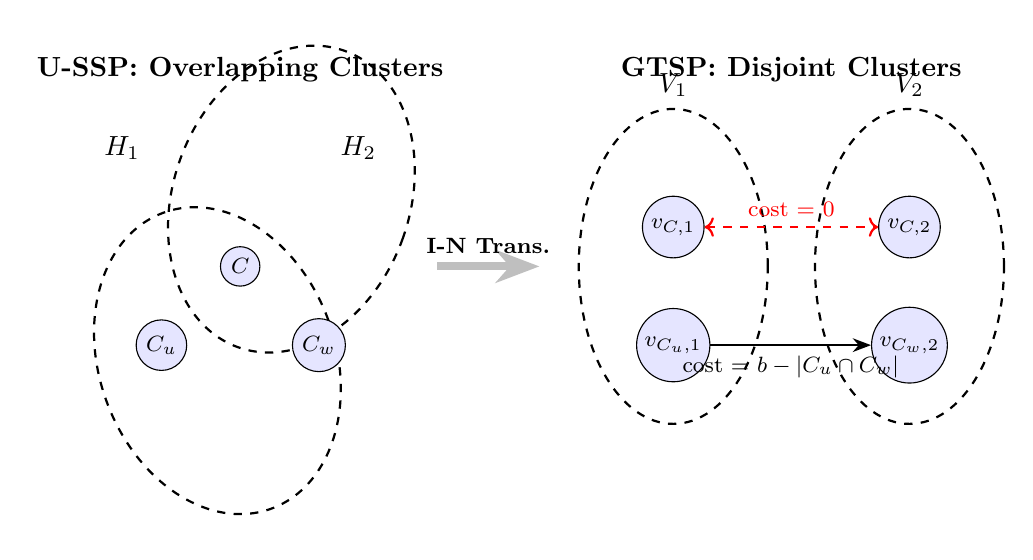
\begin{tikzpicture}[
		cluster/.style={draw, ellipse, minimum width=2.5cm, minimum height=3.5cm, dashed, thick},
		node_conf/.style={draw, circle, fill=blue!10, inner sep=2pt, font=\footnotesize},
		arrow/.style={-Stealth, thick},
		zero_arrow/.style={<->, dashed, thick, red}
		]
		
		% Left Side: SSP Overlapping
		\node[font=\bfseries] at (-3, 2.5) {U-SSP: Overlapping Clusters};
		\draw[cluster, rotate=20] (-3.5, 0) ellipse (1.5cm and 2cm);
		\draw[cluster, rotate=-20] (-2.5, 0) ellipse (1.5cm and 2cm);
		\node at (-4.5, 1.5) {$H_1$};
		\node at (-1.5, 1.5) {$H_2$};
		
		\node[node_conf] (c1) at (-3, 0) {$C$};
		\node[node_conf] (cu) at (-4, -1) {$C_u$};
		\node[node_conf] (cw) at (-2, -1) {$C_w$};
		
		% Right Side: GTSP Disjoint
		\node[font=\bfseries] at (4, 2.5) {GTSP: Disjoint Clusters};
		\draw[cluster] (2.5, 0) ellipse (1.2cm and 2cm);
		\draw[cluster] (5.5, 0) ellipse (1.2cm and 2cm);
		\node at (2.5, 2.3) {$V_1$};
		\node at (5.5, 2.3) {$V_2$};
		
		\node[node_conf] (vc1) at (2.5, 0.5) {$v_{C,1}$};
		\node[node_conf] (vu1) at (2.5, -1) {$v_{C_u,1}$};
		
		\node[node_conf] (vc2) at (5.5, 0.5) {$v_{C,2}$};
		\node[node_conf] (vw2) at (5.5, -1) {$v_{C_w,2}$};
		
		\draw[zero_arrow] (vc1) -- (vc2) node[midway, above, font=\footnotesize] {cost = 0};
		\draw[arrow] (vu1) -- (vw2) node[midway, below, font=\footnotesize] {cost = $b - |C_u \cap C_w|$};
		
		% Mapping Arrow
		\draw[-Stealth, line width=1mm, gray!50] (-0.5, 0) -- (0.8, 0) node[midway, above, text=black, font=\footnotesize\bfseries] {I-N Trans.};
		
	\end{tikzpicture}
	\caption{The Intersecting-to-Nonintersecting (I-N) transformation. A configuration $C$ capable of satisfying both Job 1 and Job 2 exists in the intersection of $H_1$ and $H_2$. In the transformed graph, $C$ is duplicated into job-specific replicas $v_{C,1}$ and $v_{C,2}$ in strictly disjoint clusters, connected by a zero-cost edge.}
	\label{fig:in_transform}
\end{figure}


\begin{lemma}[Non-Redundant Subtours]
	If a GTSP tour visits two replicas of the same configuration non-consecutively, it can always be transformed into a non-redundant tour of equal or lesser cost where all replicas of that configuration are visited consecutively.
\end{lemma}
\begin{proof}
	Let $v_{C, i}$ and $v_{C, j}$ be replicas of the same configuration $C$. Their internal distance is $d'(v_{C,i}, v_{C,j}) = b - |C \cap C| = 0$. Because the distance metric intrinsically satisfies the triangle inequality (Lemma 2.1), bypassing intermediate nodes to visit $v_{C, j}$ immediately after $v_{C, i}$ via the zero-cost edge will never increase the total tour cost. Repeated shortcutting groups all replicas of $C$ into a continuous zero-cost subtour \citep{Lien1993}.
\end{proof}

\begin{theorem}[Optimal Solution Correspondence]
	A minimum-cost GTSP tour on the transformed graph corresponds to an optimal U-SSP sequence without loss of optimality.
\end{theorem}
\begin{proof}
	By Lemma 3.1, an optimal GTSP tour can be made non-redundant. In a non-redundant tour, all replicas of a chosen configuration $C$ are visited consecutively, incurring an internal transition cost of 0 between them. This perfectly emulates the Keep Tool Needed Soonest (KTNS) policy, which retains tool configurations across a 0-block of jobs at zero penalty \citep{Tang1988}. Consequently, this non-redundant sequence of disjoint clusters collapses directly into a valid, sequence-preserving tool-loading policy for the U-SSP with identical cost.
\end{proof}

\textbf{Complexity of the Transformation:} While the I-N transformation establishes a theoretical correspondence, it is critical to quantify its algorithmic complexity. The maximum number of valid configurations is $\binom{m}{b}$. Replicating these across $n$ jobs yields a transformed state space strictly bounded by $\mathcal{O}(n \binom{m}{b})$. Because this state-space expansion requires exponential time and space, it operates as an algorithmic formulation technique for routing solvers rather than a polynomial-time Karp reduction.

\subsection{Theoretical Equivalence and Structural Subsumption}

To investigate whether the U-SSP and GTSP are strictly equivalent complexity classes, one must analyze the reverse mapping: converting a GTSP into the U-SSP.

\textbf{The Restricted Reverse Construction:} A reverse mapping is theoretically possible under highly restricted conditions. If a GTSP instance possesses strictly integer, symmetric, and Euclidean edge weights, it can be mapped to the U-SSP by artificially engineering dummy tools.

\begin{lemma}[Dummy Tool Padding]
	For any symmetric GTSP edge weight $w_{uv} \in \mathbb{Z}^+$ bounded by $b$, there exists a theoretical U-SSP configuration space where the transition cost matches the edge weight: $b - |C_u \cap C_v| = w_{uv}$.
\end{lemma}
\begin{proof}
	If we assign a unique, disjoint set of $w_{uv}$ dummy tools to configurations $C_u$ and $C_v$, while filling their remaining $b - w_{uv}$ slots with identical shared tools, the resulting set intersection is exactly $|C_u \cap C_v| = b - w_{uv}$. Applying the transition formula yields $b - (b - w_{uv}) = w_{uv}$, perfectly matching the edge weight.
\end{proof}

\begin{figure}[h!]
	\centering
	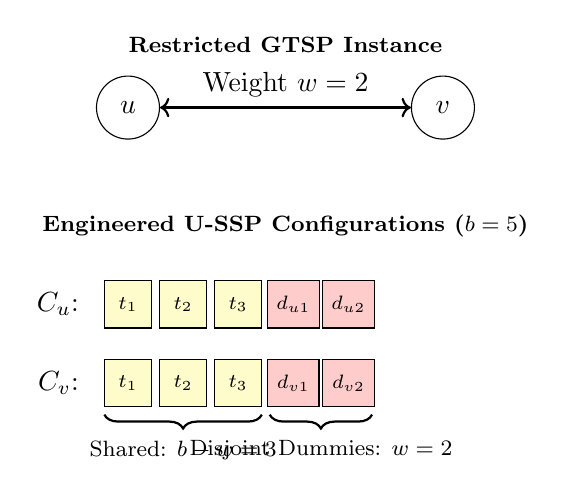
\begin{tikzpicture}[
		node_style/.style={draw, circle, minimum size=0.8cm, font=\bfseries},
		tool/.style={draw, rectangle, fill=yellow!20, minimum width=0.6cm, minimum height=0.6cm, font=\scriptsize},
		dummy/.style={draw, rectangle, fill=red!20, minimum width=0.6cm, minimum height=0.6cm, font=\scriptsize},
		arrow/.style={-Stealth, thick}
		]
		
		% GTSP Edge
		\node[node_style] (u) at (0, 2) {$u$};
		\node[node_style] (v) at (4, 2) {$v$};
		\draw[<->, thick] (u) -- (v) node[midway, above] {Weight $w = 2$};
		\node[font=\footnotesize\bfseries] at (2, 2.8) {Restricted GTSP Instance};
		
		% SSP Configurations
		\node[font=\footnotesize\bfseries] at (2, 0.5) {Engineered U-SSP Configurations ($b=5$)};
		
		\node[left] at (-0.5, -0.5) {$C_u$:};
		\node[tool] at (0, -0.5) {$t_1$};
		\node[tool] at (0.7, -0.5) {$t_2$};
		\node[tool] at (1.4, -0.5) {$t_3$};
		\node[dummy] at (2.1, -0.5) {$d_{u1}$};
		\node[dummy] at (2.8, -0.5) {$d_{u2}$};
		
		\node[left] at (-0.5, -1.5) {$C_v$:};
		\node[tool] at (0, -1.5) {$t_1$};
		\node[tool] at (0.7, -1.5) {$t_2$};
		\node[tool] at (1.4, -1.5) {$t_3$};
		\node[dummy] at (2.1, -1.5) {$d_{v1}$};
		\node[dummy] at (2.8, -1.5) {$d_{v2}$};
		
		\draw[thick, decoration={brace, amplitude=5pt}, decorate] (1.7, -1.9) -- (-0.3, -1.9) node[midway, below, yshift=-0.2cm, font=\footnotesize] {Shared: $b - w = 3$};
		\draw[thick, decoration={brace, amplitude=5pt}, decorate] (3.1, -1.9) -- (1.8, -1.9) node[midway, below, yshift=-0.2cm, font=\footnotesize] {Disjoint Dummies: $w = 2$};
	\end{tikzpicture}
	\caption{The theoretical restricted reverse construction. By generating disjoint dummy tools for specific configurations, the U-SSP transition metric $b - |C_u \cap C_v|$ can be artificially engineered to match integer GTSP edge weights. This construction requires exponential time to encode a full graph.}
	\label{fig:dummy_tools}
\end{figure}



\textbf{The Metric Barrier:} While Lemma 3.3 demonstrates a mapping, a general polynomial reduction from the GTSP to the \textbf{U-SSP} is mathematically impossible. The barrier lies in the fundamental nature of the transition costs. As established, the U-SSP's transition metric ($b - |C_u \cap C_v|$) is strictly integer-bounded, inherently symmetric, and naturally satisfies the triangle inequality. In stark contrast, a general GTSP allows for arbitrary, real-valued, and highly asymmetric edge weights. It is mathematically impossible to polynomially construct dummy tools whose set intersections can capture arbitrary real-valued metrics. However, it is worth noting that the Tool-Dependent SSP (TD-SSP) variant, which is often modeled as a max-flow min-cost network \citep{Privault1995}, \textit{can} absorb asymmetric transition costs, foreshadowing its higher complexity.

Because a general reverse reduction is prohibited by the metric barrier, the formal complexity hierarchy between the two problems is established not by artificial graph transformations, but by structural subsumption. The GTSP can be seen as a particular case of the Tool Switching Problem where the clusters $H_j$ are all disjoint \citep{Colares2026}. We formally prove that this disjointness condition occurs naturally without any artificial edge-weight mapping.

\begin{proposition}[The Disjointness Condition]
	If the union of the required tools for any two distinct jobs $i, j \in J$ strictly exceeds the magazine capacity, i.e., $|T_i \cup T_j| > b$, then their corresponding configuration clusters $H_i$ and $H_j$ are strictly disjoint ($H_i \cap H_j = \emptyset$).
\end{proposition}
\begin{proof}
	Suppose, for the sake of contradiction, that $|T_i \cup T_j| > b$ holds, yet the clusters are not disjoint ($H_i \cap H_j \neq \emptyset$). This implies there exists at least one valid tool configuration $C \in \mathcal{C}$ such that $C \in H_i$ and $C \in H_j$. By definition of the clusters, this requires $T_i \subseteq C$ and $T_j \subseteq C$. It mathematically follows that their union must also be a subset of the configuration: $(T_i \cup T_j) \subseteq C$. Consequently, the cardinality must satisfy $|T_i \cup T_j| \le |C|$. Since every valid configuration is strictly bounded by the magazine capacity ($|C| = b$), we arrive at $|T_i \cup T_j| \le b$. This directly contradicts the initial premise that $|T_i \cup T_j| > b$.
\end{proof}

Having established the structural subsumption and the continuous routing equivalence of the U-SSP to the GTSP, we have fully defined the state space required for an exact solver. We now turn to the problem of generating the discrete maximal configurations that populate this state space, exploring the tight mathematical bounds provided by the Job Grouping Problem (JGP).

\subsection{Algorithmic Implications of the Complexity Space}

Because the SSP is structurally more generalized and its forward state-space transformation (the I-N mapping) requires exponential memory, generating the complete configuration graph is only computationally viable for smaller, tightly-constrained instances. This inherent complexity dictates a bifurcated solution methodology (illustrated in Figure \ref{fig:complexity_flowchart}).

For tractable instances, the complete GTSP graph and its mutually exclusive clusters can be generated in memory. We then apply the Noon-Bean transformation \citep{Noon1993}, a graph transformation that modifies the edge weights to compel any optimal routing algorithm to visit exactly one node per cluster. This collapses the generalized problem into a standard Asymmetric Traveling Salesman Problem (ATSP), which can be solved optimally using state-of-the-art routing heuristics such as LKH-3 \citep{Helsgaun2015}.

However, for massive industrial instances where the combination of $m$ and $b$ triggers out-of-memory failures, exactness requires bypassing the full graph via dynamic node generation in a Branch-and-Price paradigm.

\begin{figure}[h!]
	\centering
	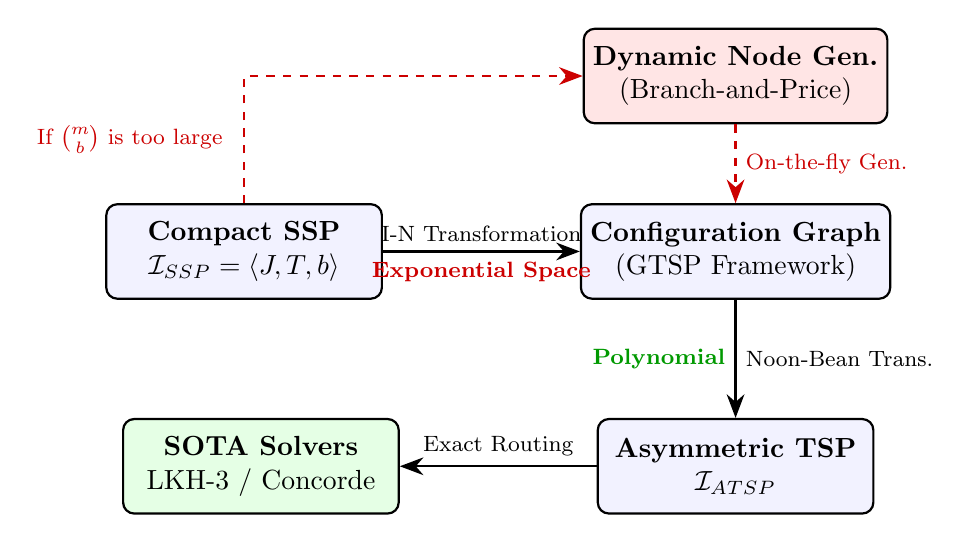
\begin{tikzpicture}[
		node distance=1.5cm and 2.5cm,
		box/.style={draw, rectangle, rounded corners, minimum width=3.5cm, minimum height=1.2cm, align=center, fill=blue!5, thick},
		arrow/.style={-{Stealth[length=3mm]}, thick}
		]
		
		% Nodes
		\node[box] (ssp) {\textbf{Compact SSP} \\ $\mathcal{I}_{SSP} = \langle J, T, b \rangle$};
		
		\node[box, right=of ssp] (gtsp) {\textbf{Configuration Graph} \\ (GTSP Framework)};
		
		\node[box, below=of gtsp] (atsp) {\textbf{Asymmetric TSP} \\ $\mathcal{I}_{ATSP}$};
		
		\node[box, fill=green!10, left=of atsp] (solvers) {\textbf{SOTA Solvers} \\ LKH-3 / Concorde};
		
		\node[box, fill=red!10, above=of gtsp, yshift=-0.5cm] (bp) {\textbf{Dynamic Node Gen.} \\ (Branch-and-Price)};
		
		% Arrows
		\draw[arrow] (ssp) -- node[above, font=\footnotesize] {I-N Transformation} node[below, font=\footnotesize\bfseries, text=red!80!black] {Exponential Space} (gtsp);
		
		\draw[arrow] (gtsp) -- node[right, font=\footnotesize] {Noon-Bean Trans.} node[left, font=\footnotesize\bfseries, text=green!60!black] {Polynomial} (atsp);
		
		\draw[arrow] (atsp) -- node[above, font=\footnotesize] {Exact Routing} (solvers);
		
		\draw[arrow, dashed, red!80!black] (ssp) |- node[near start, left, font=\footnotesize, text width=2.5cm] {If $\binom{m}{b}$ is too large} (bp);
		\draw[arrow, dashed, red!80!black] (bp) -- node[right, font=\footnotesize] {On-the-fly Gen.} (gtsp);
		
	\end{tikzpicture}
	\caption{The complexity space of solving the SSP. Tractable instances can be reduced to ATSP and solved via highly optimized routing solvers. Massive instances bypass the exponential bottleneck via dynamic node generation in a Branch-and-Price framework.}
	\label{fig:complexity_flowchart}
\end{figure}


\section{Relationship with the Job Grouping Problem (JGP)}
\label{sec:jgp_bounds}

\subsection{Conceptual Distinction and Suboptimality of JGP}

The JGP aims to partition a set of jobs into the minimum number of feasible groups such that all jobs within a group can be processed with a single setup of the tool magazine. It assumes the machine is completely halted between groups to allow for simultaneous, batch tool swaps. In contrast, the Uniform SSP (U-SSP) seeks to determine a continuous processing sequence that minimizes individual tool switches, dynamically retaining unneeded tools across transitions via policies such as the Keep Tool Needed Soonest (KTNS) rule \cite{Tang1988}.

Because the JGP forces jobs into rigid batches, it locks the magazine configuration for the duration of the group. This rigidity can temporarily choke the magazine capacity and force the unnecessary eviction of tools that will be required shortly after, leading to strict suboptimality when evaluated under continuous transitions. It is crucial to distinguish this from the Tool-Dependent SSP (TD-SSP), where asymmetric setup costs often make full batching mathematically optimal \cite{Crama1994}. However, for the U-SSP, rigid batching is strictly suboptimal.

To prove this, consider an instance with a magazine capacity of $b = 3$, containing 6 jobs and 6 tools that form a cyclical requirement ring:
\begin{itemize}[noitemsep]
	\item $T_1 = \{t_1, t_2\}$
	\item $T_2 = \{t_2, t_3\}$
	\item $T_3 = \{t_3, t_4\}$
	\item $T_4 = \{t_4, t_5\}$
	\item $T_5 = \{t_5, t_6\}$
	\item $T_6 = \{t_6, t_1\}$
\end{itemize}

The strict objective of the JGP is to partition the jobs into a minimum number of feasible groups. Because every 3 consecutive jobs require 4 distinct tools (e.g., $T_1 \cup T_2 \cup T_3 = \{t_1, t_2, t_3, t_4\}$), no 3 jobs can fit into a single group. The absolute minimum number of groups is 3 batches of 2 jobs each:
\begin{enumerate}[noitemsep]
	\item \textbf{Batch 1 (Jobs 1 \& 2):} Requires configuration $\{t_1, t_2, t_3\}$.
	\item \textbf{Batch 2 (Jobs 3 \& 4):} Requires configuration $\{t_3, t_4, t_5\}$.
	\item \textbf{Batch 3 (Jobs 5 \& 6):} Requires configuration $\{t_1, t_5, t_6\}$.
\end{enumerate}

Evaluating the continuous transition cost between these rigid JGP batches:
\begin{itemize}[noitemsep]
	\item \textbf{B1 $\to$ B2:} The magazine transitions from $\{t_1, t_2, t_3\}$ to $\{t_3, t_4, t_5\}$. Tools $t_1$ and $t_2$ are dropped to load $t_4$ and $t_5$ (2 switches).
	\item \textbf{B2 $\to$ B3:} The magazine transitions from $\{t_3, t_4, t_5\}$ to $\{t_1, t_5, t_6\}$. Tools $t_3$ and $t_4$ are dropped to load $t_1$ and $t_6$ (2 switches).
\end{itemize}

The total cost of the JGP grouping is 4 tool switches. During the transition from B1 to B2, the rigid batch requirement of Batch 2 completely fills the magazine, forcing tool $t_1$ out, even though it is required for Batch 3.

Conversely, if the U-SSP processes the same sequence of jobs sequentially using the dynamic KTNS policy, the configuration shifts continuously:
\begin{itemize}[noitemsep]
	\item \textbf{Job 1 to Job 2:} Magazine remains $\{t_1, t_2, t_3\}$ (0 switches).
	\item \textbf{Job 3:} The magazine drops $t_2$ (never needed again) and loads $t_4$. Magazine becomes $\{t_1, t_3, t_4\}$ (1 switch). Tool $t_1$ is safely retained.
	\item \textbf{Job 4:} Drops $t_3$, loads $t_5$. Magazine becomes $\{t_1, t_4, t_5\}$ (1 switch).
	\item \textbf{Job 5:} Drops $t_4$, loads $t_6$. Magazine becomes $\{t_1, t_5, t_6\}$ (1 switch).
	\item \textbf{Job 6:} Magazine is already $\{t_1, t_5, t_6\}$. Requirements are met (0 switches).
\end{itemize}

The total U-SSP cost is \textbf{3 tool switches}. By dynamically shifting the configuration and safely retaining tool $t_1$ in the corner of the magazine, the U-SSP bypasses the rigid capacity choke of the JGP, proving that $Cost_{switches}(\text{U-SSP}) \le Cost_{switches}(\text{JGP})$.

\begin{figure}[h!]
	\centering
	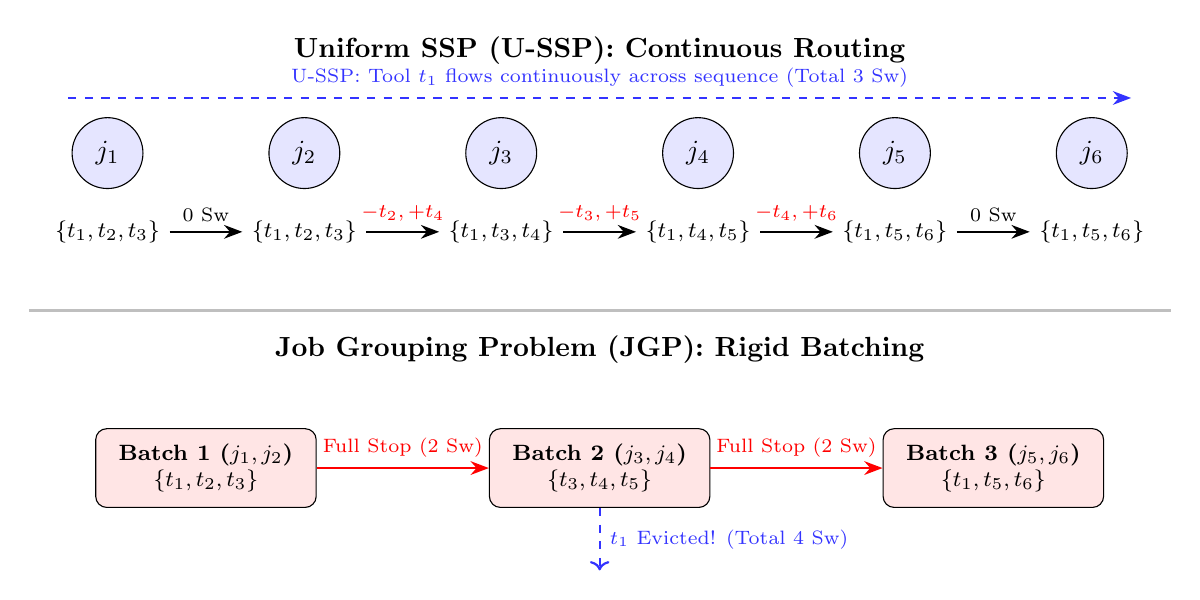
\begin{tikzpicture}[
		jobnode/.style={draw, circle, fill=blue!10, minimum size=0.9cm, font=\bfseries},
		confignode/.style={draw, rectangle, rounded corners, fill=red!10, minimum width=2.8cm, minimum height=1cm, align=center, font=\footnotesize\bfseries},
		arrow/.style={-Stealth, thick},
		swap/.style={-Stealth, thick, red},
		flow/.style={-Stealth, thick, blue!80, dashed}
		]
		
		% U-SSP Panel
		\node[font=\bfseries] at (6.25, 4.8) {Uniform SSP (U-SSP): Continuous Routing};
		
		% Jobs
		\node[jobnode] (j1) at (0, 3.5) {$j_1$};
		\node[jobnode] (j2) at (2.5, 3.5) {$j_2$};
		\node[jobnode] (j3) at (5, 3.5) {$j_3$};
		\node[jobnode] (j4) at (7.5, 3.5) {$j_4$};
		\node[jobnode] (j5) at (10, 3.5) {$j_5$};
		\node[jobnode] (j6) at (12.5, 3.5) {$j_6$};
		
		% Magazine States for U-SSP
		\node[font=\footnotesize, align=center] (m1) at (0, 2.5) {$\{t_1, t_2, t_3\}$};
		\node[font=\footnotesize, align=center] (m2) at (2.5, 2.5) {$\{t_1, t_2, t_3\}$};
		\node[font=\footnotesize, align=center] (m3) at (5, 2.5) {$\{t_1, t_3, t_4\}$};
		\node[font=\footnotesize, align=center] (m4) at (7.5, 2.5) {$\{t_1, t_4, t_5\}$};
		\node[font=\footnotesize, align=center] (m5) at (10, 2.5) {$\{t_1, t_5, t_6\}$};
		\node[font=\footnotesize, align=center] (m6) at (12.5, 2.5) {$\{t_1, t_5, t_6\}$};
		
		% Arrows between jobs (U-SSP)
		\draw[arrow] (m1) -- (m2) node[midway, above, font=\scriptsize] {0 Sw};
		\draw[arrow] (m2) -- (m3) node[midway, above, font=\scriptsize, text=red] {$-t_2, +t_4$};
		\draw[arrow] (m3) -- (m4) node[midway, above, font=\scriptsize, text=red] {$-t_3, +t_5$};
		\draw[arrow] (m4) -- (m5) node[midway, above, font=\scriptsize, text=red] {$-t_4, +t_6$};
		\draw[arrow] (m5) -- (m6) node[midway, above, font=\scriptsize] {0 Sw};
		
		% Divider
		\draw[thick, gray!50] (-1, 1.5) -- (13.5, 1.5);
		
		% JGP Panel
		\node[font=\bfseries] at (6.25, 1.0) {Job Grouping Problem (JGP): Rigid Batching};
		
		% JGP Groups
		\node[confignode] (g1) at (1.25, -0.5) {Batch 1 ($j_1, j_2$) \\ $\{t_1, t_2, t_3\}$};
		\node[confignode] (g2) at (6.25, -0.5) {Batch 2 ($j_3, j_4$) \\ $\{t_3, t_4, t_5\}$};
		\node[confignode] (g3) at (11.25, -0.5) {Batch 3 ($j_5, j_6$) \\ $\{t_1, t_5, t_6\}$};
		
		% Swaps between groups (JGP)
		\draw[swap] (g1) -- (g2) node[midway, above, font=\scriptsize] {Full Stop (2 Sw)};
		\draw[swap] (g2) -- (g3) node[midway, above, font=\scriptsize] {Full Stop (2 Sw)};
		
		% Tool t1 retention flow comparison
		\draw[flow] (-0.5, 4.2) -- (13, 4.2) node[midway, above, font=\scriptsize] {U-SSP: Tool $t_1$ flows continuously across sequence (Total 3 Sw)};
		\draw[flow, ->] (g2) -- (6.25, -1.8) node[midway, right, font=\scriptsize] {$t_1$ Evicted! (Total 4 Sw)};
		
	\end{tikzpicture}
	\caption{Graph-theoretic contrast between the Job Grouping Problem (JGP) and the Uniform Tool Switching Problem (U-SSP). The JGP acts as a Set Covering problem, mapping jobs to rigid, independent configuration nodes separated by full machine stops where $t_1$ is unnecessarily evicted. The U-SSP models a continuous routing path, evaluating dynamic edge costs via KTNS and allowing $t_1$ to flow seamlessly across the sequence.}
	\label{fig:6job_ring}
\end{figure}


\subsection{Approximation Bounds from JGP to U-SSP}

While an optimal JGP solution cannot guarantee an optimal U-SSP sequence, it provides a strict and reliable theoretical upper bound. We can mathematically establish that the optimal JGP solution yields an $\alpha$-approximation for the U-SSP, where $\alpha = b$ (the magazine capacity).

\begin{theorem}[$\alpha$-Approximation]
	Let $Cost_{groups}(\text{JGP})$ be the minimum number of groups (machine stops) required to partition the jobs such that no group exceeds the magazine capacity $b$. Let $Cost_{switches}(\text{U-SSP})$ be the minimum number of individual tool switches required to process the jobs continuously. Then, the following bound strictly holds:
	\begin{equation}
		Cost_{switches}(\text{U-SSP}) \le b \cdot Cost_{groups}(\text{JGP})
	\end{equation}
\end{theorem}
\begin{proof}
	Assume the JGP optimally partitions the job sequence into $k = Cost_{groups}(\text{JGP})$ disjoint groups: $G_1, G_2, \dots, G_k$. By the definition of the JGP, each group $G_i$ requires a set of tools $T(G_i)$ such that $|T(G_i)| \le b$. 
	
	If we sequence the jobs exactly according to this grouping ($G_1 \to G_2 \to \dots \to G_k$), the machine must undergo a setup between each group. In the absolute worst-case scenario, the tool requirements for consecutive groups are entirely disjoint ($T(G_i) \cap T(G_{i+1}) = \emptyset$). If this worst-case disjointness occurs, the machine must flush the entire magazine and load exactly $b$ new tools during the transition. 
	
	Since there are exactly $k$ groups, there are exactly $k - 1$ transitions between them. The initial loading of the magazine at the start of $G_1$ requires at most $b$ tool insertions. Therefore, the maximum number of individual tool switches across the entire rigid sequence is bounded by:
	\begin{equation}
		\text{Total Switches} \le b + b(k - 1) = b \cdot k
	\end{equation}
	Substituting our initial definitions, we obtain an upper bound for the switches incurred by the rigid JGP grouping:
	\begin{equation}
		Cost_{switches}(\text{JGP}) \le b \cdot Cost_{groups}(\text{JGP})
	\end{equation}
	From Section 4.1, we established that evaluating the exact same sequence with the continuous KTNS policy guarantees $Cost_{switches}(\text{U-SSP}) \le Cost_{switches}(\text{JGP})$ by successfully flipping 0-blocks. Transitivity directly yields our final bound:
	\begin{equation}
		Cost_{switches}(\text{U-SSP}) \le Cost_{switches}(\text{JGP}) \le b \cdot Cost_{groups}(\text{JGP})
	\end{equation}
	Thus, the optimal JGP objective multiplied by the capacity $b$ serves as a strict upper bound (an $\alpha$-approximation where $\alpha=b$) for the U-SSP objective.
\end{proof}

\subsection{Lower Bounds and Polyhedral Cutting Planes}

While Theorem 4.1 establishes that the JGP provides a reliable upper bound on the number of tool switches, an exact solution to the U-SSP requires tight lower bounds to effectively prune the search space. Historically, finding strong lower bounds for the U-SSP was a severe computational bottleneck because the linear relaxation of early compact ILP models often yielded a weak lower bound of exactly zero. To overcome this, modern exact approaches rely on state-space bounds and polyhedral cutting planes.

\textbf{Capacity and Routing Bounds:} When constructing a partial sequence of jobs, look-ahead bounds can be dynamically computed to estimate the minimum number of remaining tool switches. \cite{Laporte2004} introduced two highly effective bounding mechanisms evaluated over the set of unassigned jobs:
\begin{enumerate}
	\item \textbf{The Capacity Bound (LB1):} This bound evaluates the absolute minimum number of tool insertions required to finish the sequence. It is calculated as the total number of unique tools required by all remaining jobs (and not present in the last completed job's toolset), minus the number of currently free slots in the magazine. Mathematically, it is the cardinality of the required remaining tools minus the capacity $b$ \cite{Laporte2004}.
	\item \textbf{The Spanning Tree Bound (LB2):} Because the U-SSP entails a routing component, a valid lower bound on the remaining transition costs can be derived by constructing a minimum spanning tree over the remaining unassigned jobs, utilizing the transition cost metric between their respective required toolsets \cite{Laporte2004}. 
\end{enumerate}
In a branch-and-bound framework, taking the maximum of these two bounds (or summing them under specific conditions) provides a significantly tighter lower bound than the continuous linear relaxation.

\textbf{GTSP Cutting Planes:} Because we have formally mapped the U-SSP to the GTSP configuration graph (as demonstrated in Section 3), we can directly exploit the tight bounds of the GTSP polytope to strengthen the root node relaxation. The most powerful of these polyhedral cuts are the Generalized Subtour Elimination Constraints (GSECs) \cite{Fischetti1997}. 

By separating and adding violated GSECs at the root node of a Branch-and-Cut algorithm, the formulation strictly forbids disconnected fractional sub-cycles among the configuration clusters. \cite{Fischetti1997} demonstrated that identifying these violated GSECs via maximum flow separation algorithms and adding them as cutting planes pushes the lower bound extremely close to the optimal integer solution, effectively shattering the "zero-bound" barrier that plagued early compact formulations.

While these exact bounding mechanisms are robust, they rely on having a fully populated state space of valid maximal configurations. Generating these configuration vertices dynamically introduces a profound computational hurdle, inextricably linking the continuous U-SSP back to the subset selection logic of the JGP. We now turn to this bottleneck.

\section{Dynamic Node Generation and the Pricing Oracle}
\label{sec:pricing_oracle}

As established in Section 3.4, for industrial instances where enumerating the full state space of $\binom{m}{b}$ configurations is intractable, the GTSP configuration graph must be populated dynamically. This section formally dissects the mathematical nature of this dynamic generation process, strictly differentiating the routing formulation of the U-SSP from traditional column generation schemes, and exposing the severe computational bottleneck that justifies our machine learning interventions.

\subsection{Differentiating the Pricing Oracles: SPPRC vs. SUKP}

In standard routing problems solved via Branch-and-Price, such as the Vehicle Routing Problem (VRP) or the Prize-Collecting TSP (PCTSP), the Restricted Master Problem (RMP) selects among a pool of \textit{full routes} \cite{Barnhart1998} [1]. Consequently, the pricing subproblem responsible for generating a new column (route) with a negative reduced cost must simultaneously maximize collected dual variables and minimize the continuous routing costs along the edges [2]. This subproblem is universally modeled as the Shortest Path Problem with Resource Constraints (SPPRC) [1].

However, the non-compact formulation of the U-SSP does not generate full routes as columns. Instead, it generates individual \textit{configuration vertices} to incrementally build the GTSP graph. Because adding a new configuration vertex $v$ to the RMP simultaneously requires adding new transition edges $x(u,v)$ connecting it to all existing vertices, this architecture mathematically necessitates Simultaneous Column-and-Row Generation \cite{Muter2013} [3].

Within this framework, to generate a promising new configuration vertex that satisfies the covering constraints of the RMP, the pricing oracle evaluates the dual variables $\pi_j$ associated with each job $j \in J$ [4, 5]. The oracle seeks to find a single valid tool configuration of size $b$ that maximizes the sum of the dual variables for the jobs it can completely process. Because the transition edge costs $d(u,v)$ are only evaluated in the master routing problem once the node is generated, the node-generation oracle itself does not evaluate routing costs.

This subproblem—finding a subset of tools bounded by a capacity constraint to maximize the profit of satisfied jobs—is mathematically identical to the pricing subproblem of the Job Grouping Problem (JGP). As demonstrated by Crama and Oerlemans \cite{Crama1994} [6, 7], and formally classified in recent literature, this oracle is exactly the Set Union Knapsack Problem (SUKP) \cite{Goldschmidt1994} [7].

\subsection{Formalizing the SUKP Pricing Oracle}

Let $y_j \in \{0,1\}$ be a binary variable indicating whether job $j \in J$ is covered by the new configuration [6]. Let $z_t \in \{0,1\}$ be a binary variable indicating whether tool $t \in T$ is included in the magazine [6]. Given the dual variables $\pi_j \ge 0$ obtained from the RMP's job-covering constraints, the SUKP pricing oracle for the U-SSP is formulated as:

\begin{align}
	\max \quad & \sum_{j \in J} \pi_j y_j \label{eq:sukp_obj} \\
	\text{subject to} \quad & \sum_{t \in T} z_t = b \label{eq:sukp_cap} \\
	& y_j \le z_t, \quad \forall j \in J, \forall t \in T_j \label{eq:sukp_link} \\
	& y_j \in \{0,1\}, \quad \forall j \in J \label{eq:sukp_y} \\
	& z_t \in \{0,1\}, \quad \forall t \in T \label{eq:sukp_z}
\end{align}

The objective (\ref{eq:sukp_obj}) maximizes the collected dual variables associated with the covered jobs [8]. Constraint (\ref{eq:sukp_cap}) strictly enforces the maximal configuration property under the U-SSP assumption by filling the magazine capacity $b$ [8]. The logical linking constraints (\ref{eq:sukp_link}) ensure that a job $j$ can only be claimed as covered ($y_j = 1$) if every single tool $t$ required by that job ($t \in T_j$) is currently loaded in the magazine ($z_t = 1$) [8].

\section{Relationship with the Job Grouping Problem (JGP)}

To fully contextualize the non-compact formulation and the necessity of dynamic column generation for the SSP, it is critical to establish its relationship with the Job Grouping Problem (JGP). Historically, Column Generation in flexible manufacturing was pioneered to solve the JGP by treating it as a Set Covering problem, where each generated column represents a feasible tool configuration capable of processing a subset of jobs \citep{Crama1994}. 

While the SSP's Restricted Master Problem (RMP) utilizes these exact same generated configurations as its vertices, the fundamental objectives and transition mechanics of the two problems differ significantly, which justifies why a pure JGP solution is insufficient for the SSP.

\subsection{Conceptual Distinction and Suboptimality of JGP}

The JGP aims to partition a set of jobs into the minimum number of feasible groups such that all jobs within a group can be processed with a single setup of the tool magazine. It assumes the machine is completely halted between groups to allow for simultaneous, batch tool swaps. In contrast, the SSP seeks to determine a continuous processing sequence that minimizes individual tool switches, dynamically retaining unneeded tools across transitions via policies such as the Keep Tool Needed Soonest (KTNS) rule \citep{Tang1988}.

Because the JGP forces jobs into rigid batches, it locks the magazine configuration for the duration of the group. This rigidity can temporarily choke the magazine capacity and force the unnecessary eviction of tools that will be required shortly after, leading to strict suboptimality when evaluated under continuous transitions.

To prove this, consider an instance with a magazine capacity of $b = 3$, containing 6 jobs and 6 tools that form a cyclical requirement ring:
\begin{itemize}[noitemsep]
	\item $T_1 = \{t_1, t_2\}$
	\item $T_2 = \{t_2, t_3\}$
	\item $T_3 = \{t_3, t_4\}$
	\item $T_4 = \{t_4, t_5\}$
	\item $T_5 = \{t_5, t_6\}$
	\item $T_6 = \{t_6, t_1\}$
\end{itemize}

The strict objective of the JGP is to partition the jobs into a minimum number of feasible groups. Because every 3 consecutive jobs require 4 distinct tools (e.g., $T_1 \cup T_2 \cup T_3 = \{t_1, t_2, t_3, t_4\}$), no 3 jobs can fit into a single group. The absolute minimum number of groups is 3 batches of 2 jobs each:
\begin{enumerate}[noitemsep]
	\item \textbf{Group 1 (Jobs 1 \& 2):} Requires configuration $\{t_1, t_2, t_3\}$.
	\item \textbf{Group 2 (Jobs 3 \& 4):} Requires configuration $\{t_3, t_4, t_5\}$.
	\item \textbf{Group 3 (Jobs 5 \& 6):} Requires configuration $\{t_1, t_5, t_6\}$.
\end{enumerate}

Evaluating the continuous transition cost between these rigid JGP batches:
\begin{itemize}[noitemsep]
	\item \textbf{G1 $\to$ G2:} The magazine transitions from $\{t_1, t_2, t_3\}$ to $\{t_3, t_4, t_5\}$. Tools $t_1$ and $t_2$ are dropped to load $t_4$ and $t_5$ (2 switches).
	\item \textbf{G2 $\to$ G3:} The magazine transitions from $\{t_3, t_4, t_5\}$ to $\{t_1, t_5, t_6\}$. Tools $t_3$ and $t_4$ are dropped to load $t_1$ and $t_6$ (2 switches).
\end{itemize}
The total cost of the JGP grouping is \textbf{4 tool switches}. During the transition from G1 to G2, the rigid batch requirement of Group 2 completely fills the magazine, forcing tool $t_1$ out, even though it is required for Group 3.

Conversely, if the SSP processes the same sequence of jobs sequentially using the dynamic KTNS policy, the configuration shifts continuously:
\begin{itemize}[noitemsep]
	\item \textbf{Job 1 to Job 2:} Magazine remains $\{t_1, t_2, t_3\}$ (0 switches).
	\item \textbf{Job 3:} The magazine drops $t_2$ (never needed again) and loads $t_4$. Magazine becomes $\{t_1, t_3, t_4\}$ (1 switch). Tool $t_1$ is safely retained.
	\item \textbf{Job 4:} Drops $t_3$, loads $t_5$. Magazine becomes $\{t_1, t_4, t_5\}$ (1 switch).
	\item \textbf{Job 5:} Drops $t_4$, loads $t_6$. Magazine becomes $\{t_1, t_5, t_6\}$ (1 switch).
	\item \textbf{Job 6:} Magazine is already $\{t_1, t_5, t_6\}$. Requirements are met (0 switches).
\end{itemize}
The total SSP cost is \textbf{3 tool switches}. By dynamically shifting the configuration and safely retaining tool $t_1$ in the corner of the magazine, the SSP bypasses the rigid capacity choke of the JGP, proving that $Cost_{switches}(SSP) \le Cost_{switches}(JGP)$.


\begin{figure}[h!]
	\centering
	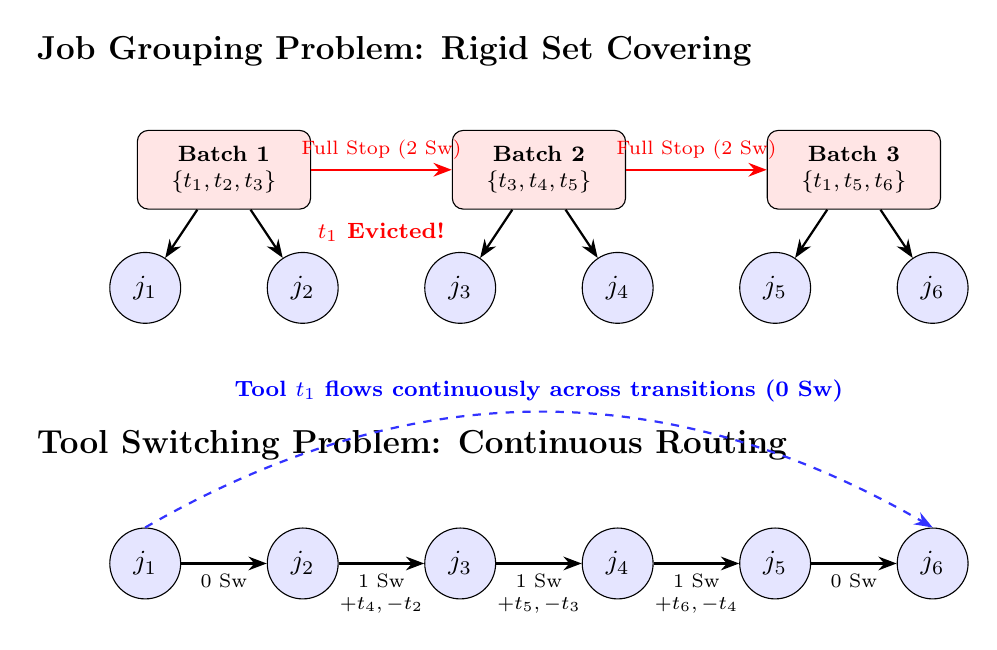
\begin{tikzpicture}[
		jobnode/.style={draw, circle, fill=blue!10, minimum size=0.9cm, font=\bfseries},
		confignode/.style={draw, rectangle, rounded corners, fill=red!10, minimum width=2.2cm, minimum height=1cm, align=center, font=\footnotesize\bfseries},
		arrow/.style={-Stealth, thick},
		swap/.style={-Stealth, thick, red},
		flow/.style={-Stealth, thick, blue!80, dashed}
		]
		
		% ----- JGP: Set Covering -----
		\node[font=\large\bfseries, anchor=west] at (-1, 3.5) {Job Grouping Problem: Rigid Set Covering};
		
		% Config Nodes
		\node[confignode] (c1) at (1.5, 2) {Batch 1 \\ $\{t_1, t_2, t_3\}$};
		\node[confignode] (c2) at (5.5, 2) {Batch 2 \\ $\{t_3, t_4, t_5\}$};
		\node[confignode] (c3) at (9.5, 2) {Batch 3 \\ $\{t_1, t_5, t_6\}$};
		
		% Job Nodes
		\node[jobnode] (j1) at (0.5, 0.5) {$j_1$};
		\node[jobnode] (j2) at (2.5, 0.5) {$j_2$};
		\draw[arrow] (c1) -- (j1); \draw[arrow] (c1) -- (j2);
		
		\node[jobnode] (j3) at (4.5, 0.5) {$j_3$};
		\node[jobnode] (j4) at (6.5, 0.5) {$j_4$};
		\draw[arrow] (c2) -- (j3); \draw[arrow] (c2) -- (j4);
		
		\node[jobnode] (j5) at (8.5, 0.5) {$j_5$};
		\node[jobnode] (j6) at (10.5, 0.5) {$j_6$};
		\draw[arrow] (c3) -- (j5); \draw[arrow] (c3) -- (j6);
		
		% Stop Indicators
		\draw[swap] (c1) -- (c2) node[midway, above, font=\scriptsize] {Full Stop (2 Sw)};
		\draw[swap] (c2) -- (c3) node[midway, above, font=\scriptsize] {Full Stop (2 Sw)};
		\node[red, font=\footnotesize\bfseries] at (3.5, 1.2) {$t_1$ Evicted!};
		
		% ----- SSP: Routing -----
		\node[font=\large\bfseries, anchor=west] at (-1, -1.5) {Tool Switching Problem: Continuous Routing};
		
		% Job Nodes sequence
		\node[jobnode] (s1) at (0.5, -3) {$j_1$};
		\node[jobnode] (s2) at (2.5, -3) {$j_2$};
		\node[jobnode] (s3) at (4.5, -3) {$j_3$};
		\node[jobnode] (s4) at (6.5, -3) {$j_4$};
		\node[jobnode] (s5) at (8.5, -3) {$j_5$};
		\node[jobnode] (s6) at (10.5, -3) {$j_6$};
		
		% Edges
		\draw[arrow] (s1) -- (s2) node[midway, below, font=\scriptsize] {0 Sw};
		\draw[arrow] (s2) -- (s3) node[midway, below, font=\scriptsize, align=center] {1 Sw\\$+t_4, -t_2$};
		\draw[arrow] (s3) -- (s4) node[midway, below, font=\scriptsize, align=center] {1 Sw\\$+t_5, -t_3$};
		\draw[arrow] (s4) -- (s5) node[midway, below, font=\scriptsize, align=center] {1 Sw\\$+t_6, -t_4$};
		\draw[arrow] (s5) -- (s6) node[midway, below, font=\scriptsize] {0 Sw};
		
		% Tool flow
		\draw[flow, out=30, in=150] (s1.north) to node[above, font=\footnotesize\bfseries, text=blue] {Tool $t_1$ flows continuously across transitions (0 Sw)} (s6.north);
		
	\end{tikzpicture}
	\caption{Graph-theoretic contrast between the Job Grouping Problem (JGP) and the Tool Switching Problem (SSP). The JGP acts as a Set Covering problem, mapping jobs to rigid, independent configuration nodes separated by full machine stops. The SSP models a continuous routing path, evaluating dynamic edge costs between individual jobs and allowing specific tools (such as $t_1$) to flow seamlessly across the sequence.}
	\label{fig:jgp_vs_ssp}
\end{figure}

\subsection{Approximation Bounds from JGP to SSP}

While an optimal JGP solution cannot guarantee an optimal SSP sequence, it provides a strict and reliable theoretical bound. We can mathematically establish that the optimal JGP solution yields an $\alpha$-approximation for the SSP, where $\alpha = b$ (the magazine capacity).

Let $S_{SSP}$ be the optimal number of tool switches in the SSP. Let $g_{JGP}$ be the optimal (minimum) number of groups in the JGP.

\textbf{Step 1: Bounding JGP groups using SSP switches.}
In an optimal SSP schedule, the magazine state changes exactly $S_{SSP}$ times, creating a timeline of $S_{SSP} + 1$ distinct magazine configurations. Because every job is processed entirely within one of these configurations, and every configuration strictly respects the magazine capacity $b$, these $S_{SSP} + 1$ configurations represent a valid JGP grouping. Since $g_{JGP}$ is the absolute minimum number of feasible groups required, it must mathematically hold that:
\begin{equation}
	g_{JGP} \le S_{SSP} + 1 \implies g_{JGP} - 1 \le S_{SSP}
\end{equation}

\textbf{Step 2: Bounding JGP switch cost using JGP groups.}
In the absolute worst-case scenario, transitioning between two completely disjoint JGP groups requires a complete machine stop and a total flush of the magazine, costing exactly $b$ tool switches. Because there are $g_{JGP}$ groups, there are exactly $g_{JGP} - 1$ transitions. Therefore, the maximum possible number of tool switches forced by the JGP solution is:
\begin{equation}
	Cost_{switches}(JGP) \le (g_{JGP} - 1) \times b
\end{equation}

\textbf{Step 3: The Approximation Bound.}
Substituting the inequality from Step 1 into Step 2 yields $Cost_{switches}(JGP) \le S_{SSP} \times b$. Dividing both sides by $S_{SSP}$ establishes the final bound:
\begin{equation}
	\frac{Cost_{switches}(JGP)}{S_{SSP}} \le b
\end{equation}

This deduction proves that any JGP optimal solution will always provide an $\alpha$-approximation for the SSP strictly bounded by the size of the tool magazine $b$. Consequently, the JGP Set Covering formulations serve as a highly effective initial construction phase. Modern solution frameworks can initialize their Branch-and-Price structures using these JGP configurations (columns), subsequently refining them via GTSP routing logic and metaheuristic improvement strategies to close the optimality gap.

\subsection{Tightening the Bounds: From Heuristics to Exact Methods}

While the $\alpha$-approximation establishes a theoretical worst-case guarantee, solving the SSP in practice requires aggressively closing the gap between the JGP batching formulation and the continuous SSP routing sequence. In a Branch-and-Price framework, algorithmic efficiency dictates that we establish tight upper bounds (primal bounds) to prune the search tree, and tight lower bounds (dual bounds) to prove optimality. 

\textbf{Heuristic Upper Bounds.} Because a valid JGP batching solution can be flattened into a linear job sequence, evaluating that sequence using the KTNS policy inherently provides a valid upper bound for the SSP. However, owing to the rigid batch boundaries of the JGP, this naive upper bound is rarely tight. To overcome this, early research proposed using JGP solutions merely as an initial construction phase, which is subsequently refined by improvement heuristics. Methods such as the ``Super Task'' heuristic \citep{Privault1995} and global 2-opt local search \citep{Crama1994} were deployed to break the rigid JGP batch boundaries, allowing the algorithm to rearrange jobs and exploit overlapping tool requirements. 

However, pure local search is highly susceptible to local optima. To establish the tightest heuristic upper bounds, the current state-of-the-art relies on hybrid population-based metaheuristics, such as Hybrid Genetic Search (HGS) \citep{Mecler2021} and Adaptive Large Neighborhood Search (ALNS) \citep{Beezao2017}. Alternatively, by mapping the configurations to a GTSP, highly optimized routing heuristics such as LKH-3 \citep{Helsgaun2015} can be applied to find near-optimal continuous sequences. Injecting these high-quality sequences as initial primal bounds drastically reduces the size of the exact search tree.

\textbf{Strengthening Lower Bounds.} Historically, establishing tight lower bounds for the SSP has been a severe computational bottleneck. The original Integer Linear Programming (ILP) formulations, such as those proposed by \citet{Tang1988}, suffered from notoriously weak linear relaxations. The ``zero-bound'' LP relaxation of early compact models forced branch-and-bound algorithms into nearly complete enumeration. 

Subsequent literature sought to overcome this by introducing valid inequalities. \citet{Laporte2004} significantly tightened the lower bound by adding subtour elimination constraints, alongside look-ahead capacity and spanning tree bounds. By projecting the SSP entirely onto a GTSP configuration graph, the non-compact formulation inherently bypasses the weak linear relaxations of classical models. Furthermore, it allows the Branch-and-Price framework to exploit the tight bounds of the GTSP polytope. As demonstrated by \citet{Fischetti1997}, separating and adding Generalized Subtour Elimination Constraints (GSECs) can push the lower bound extremely close to the optimal integer solution at the root node.

\textbf{The Pricing Bottleneck.} The synthesis of JGP-derived columns, metaheuristic upper bounds, and GTSP-based lower bounds provides a robust Branch-and-Price framework capable of exact SSP resolution. However, a critical barrier remains. While the JGP's pure Set Covering oracle can be solved dynamically, the pricing oracle for the continuous SSP must simultaneously maximize dual variable collection while accounting for sequence-dependent transition costs. This renders the oracle strongly NP-hard. Solving this exact pricing problem at every column generation iteration dominates the computation time, necessitating the integration of Machine Learning to intelligently accelerate column generation.


\subsection{Tool-Dependent Setup Times and Lexicographical Minimization}

In the preceding sections, we established that the Job Grouping Problem (JGP) is structurally rigid and provides only an upper bound ($\alpha$-approximation) for the uniform SSP. However, the operational reality of flexible manufacturing often involves \textit{tool-dependent setup times} (the non-uniform SSP variant), where different tools require significantly different amounts of time or human effort to load into the magazine. 

\textbf{The Failure of KTNS:}
In the uniform SSP, sequence evaluation is solved in $O(mn)$ time via the greedy Keep Tool Needed Soonest (KTNS) policy. However, as proved by \cite{Crama1994}, when setup times $b_k$ are tool-dependent, the greedy optimal substructure of KTNS collapses. Instead, the tooling subproblem must be formulated as a 0-1 Linear Program to maximize the saved setup costs of retained tools. Because the constraint matrix exhibits the consecutive ones property, it forms an \textit{interval matrix}. While interval matrices are totally unimodular and solvable in polynomial time via linear relaxation \cite{Crama1994}, executing a full LP for \textit{every} continuous sequence transition during routing renders the continuous SSP computationally devastating.

\textbf{Operational Reality and Lexicographical Minimization:}
To overcome this computational barrier, we look to practical manufacturing operations: when tool load times are highly variable, it is most efficient to halt the machine entirely and execute all necessary tool changes simultaneously in parallel. 

Let $c_{switch}$ be the average operational cost of an individual tool switch, and let $C_{stop}$ be the fixed penalty of halting the machine to execute a batch of tool swaps. Because tools are swapped in parallel during a machine halt, the duration of the halt is bounded by the maximum individual load time ($\max_k b_k$) rather than the sum of load times ($\sum b_k$). This heavily inflates the value of $C_{stop}$ relative to $c_{switch}$. 

If $C_{stop} \gg c_{switch} \times b$, the objective function transitions into a \textbf{Lexicographical Minimization} framework \cite{Adjiashvili2015}:
\begin{enumerate}[noitemsep]
	\item \textbf{Primary Objective:} Minimize the total number of full machine stops (the exact JGP Set Covering objective).
	\item \textbf{Secondary Objective:} Minimize the individual tool switches within those defined boundaries (the SSP routing objective).
\end{enumerate}

Recent literature proves that any optimal JGP stop plan can be mapped directly to a feasible, optimal tool switching plan for this primary objective \cite{Adjiashvili2015}. Therefore, when $C_{stop}$ dominates due to tool-dependent setup times, generating maximal configurations via the JGP is not merely a heuristic relaxation for the uniform SSP; it becomes the exact mathematical bound and optimal operational strategy for the non-uniform variant. 


\section{The Pricing Oracle and the Set Union Knapsack Problem}

The previous sections established a profound link between two classical Combinatorial Optimization problems: the JGP provides the structurally optimal vertices (configurations), while the GTSP routing framework evaluates the continuous transitions between them. However, generating these JGP configurations dynamically within a non-compact Branch-and-Price (B\&P) framework introduces a severe computational bottleneck in the form of the Pricing Oracle. 

In the non-compact B\&P framework, the Restricted Master Problem (RMP) selects configurations, but the \textbf{Pricing Subproblem} must iteratively generate new maximal configurations $C$ (where $|C| = b$) with negative reduced costs. Given the dual variables $\pi_i \ge 0$ obtained from the RMP's job-covering constraints, the pricing problem seeks a configuration $C$ that covers a subset of jobs $S \subseteq J$ to maximize the collected duals $\sum_{i \in S} \pi_i$, subject to the magazine capacity $|\bigcup_{i \in S} T_i| \le b$. 

\textbf{Mathematical Equivalence to the SUKP:}
This exact mathematical structure is identical to the \textbf{Set Union Knapsack Problem (SUKP)} \cite{Goldschmidt1994}. In the SUKP, items (jobs) have profits ($\pi_i$), and each item requires a set of elements (tools $T_i$). The weight of a subset of items is defined strictly by the cardinality of the union of their elements. 

The SUKP is known to be strongly NP-hard. Exact dynamic programming algorithms for solving the SUKP exhibit an exponential worst-case complexity proportional to:
\begin{equation}
	O\left(m n b \sum_{j=1}^n 2^{|h(j)|}\right)
\end{equation}
where $h(j)$ denotes the set of elements adjacent to element $j$ in the item-adjacency graph \cite{Goldschmidt1994}. 

Because the exact formulation of the SSP pricing oracle is fundamentally an SUKP, solving it to optimality at every iteration represents the primary computational barrier preventing the scalability of the exact B\&P framework. This exponential complexity barrier explicitly necessitates the development of Machine Learning-based pricing heuristics (such as Neural Column Generation or Deep Reinforcement Learning) to approximate the oracle and accelerate the solver, which we explore in the subsequent sections.






	
	\section{Exact Routing for Tractable Instances}
	
	As established by the complexity framework, generating the complete configuration graph is computationally viable only for smaller, tightly constrained instances where the combination of $m$ and $b$ does not cause the state space $\mathcal{O}(|J| \binom{m}{b})$ to exceed memory limits. For these tractable instances, we can leverage highly optimized, state-of-the-art routing solvers by applying a secondary polynomial transformation.
	
	Once the overlapping SSP clusters are expanded into mutually exclusive GTSP clusters via the I-N transformation, the problem can be reduced to a standard Asymmetric Traveling Salesman Problem (ATSP). This is achieved through the Noon-Bean transformation \citep{Noon1993}, which systematically modifies the intra-cluster and inter-cluster edge weights to logically compel any exact routing algorithm to visit exactly one node per cluster.
	
	By collapsing the generalized problem into an ATSP, the formulation can be passed directly to advanced routing heuristics and exact solvers, such as LKH-3 \citep{Helsgaun2015}. While this approach yields optimal or near-optimal solutions rapidly for small instances, its reliance on the full, explicit enumeration of the configuration graph renders it intractable for massive industrial applications, necessitating dynamic node generation.
	
	\section{Dynamic Node Generation and the True Pricing Bottleneck}
	
	For large-scale instances, the exponential size of the vertex set $V(K_p)$ makes it impossible to define the complete problem space upfront. Instead, we transition from the non-compact formulation to a Branch-and-Price paradigm. The problem is decomposed into a Restricted Master Problem (RMP), which operates over a small, generated subset of valid configuration sequences (columns), and a pricing oracle, which dynamically generates new sequences on-the-fly.
	
	The RMP is formulated as a Set Covering problem, selecting a combination of generated sequences to satisfy all job requirements at a minimal transition cost. Let $\pi_j \ge 0$ be the dual variables associated with the covering constraints of the RMP for each job $j \in J$. 
	
	The pricing oracle's objective is to find a new sequence of configurations (a column) whose inclusion in the RMP could improve the objective function. Mathematically, it must identify a sequence with a negative reduced cost $\bar{c}$. For a newly generated continuous sequence of configurations $C$, the reduced cost is calculated as:
	\begin{equation} \label{eq:reduced_cost}
		\bar{c} = \sum_{(u,v) \in E(C)} d(u,v) - \sum_{j \in J(C)} \pi_j
	\end{equation}
	where $E(C)$ represents the edges of the generated configuration sequence, $d(u,v)$ is the tool switching transition cost, and $J(C)$ is the subset of jobs covered by the sequence.
	
	\begin{proposition}[NP-Hardness of the SSP Pricing Oracle]
		The pricing problem for the non-compact SSP formulation is strongly NP-hard.
	\end{proposition}
	\begin{proof}
		The pricing oracle requires identifying a valid sequence of configurations $C \in \mathcal{C}$ that minimizes the reduced cost $\bar{c}$ defined in Equation \eqref{eq:reduced_cost}. This requires simultaneously determining an optimal subset of jobs $J(C)$ to cover (to maximize the collected dual variables $\pi_j$) while finding the shortest valid tool-switching sequence to process them (to minimize the transition costs $d(u,v)$). This structure perfectly mirrors the Prize-Collecting Traveling Salesman Problem (PCTSP), where dual variables act as collected prizes and switching costs act as routing penalties. Because the PCTSP is inherently strongly NP-hard, identifying the column with the minimum reduced cost for the SSP is also strongly NP-hard.
	\end{proof}
	
	It is crucial to distinguish this pricing oracle from the Job Grouping Problem (JGP). The JGP acts as a pure Set Union Knapsack Problem because it assumes the machine is completely halted for simultaneous batch swaps. In contrast, the sequential SSP pricing oracle must account for continuous transition costs $d(u,v)$ along the edges. Because solving this NP-hard oracle exactly via Mixed-Integer Linear Programming (MILP) at every column generation iteration dominates the total computation time, accelerating the oracle is the primary focus of our future experimental roadmap.
	
	\section{Machine Learning Interventions}
	
	To overcome the exact pricing bottleneck, we propose integrating Machine Learning (ML) techniques at critical stages of the Branch-and-Price algorithm. By substituting expensive exact computations with rapid, learned approximations, we can accelerate convergence while maintaining global optimality guarantees.
	
	\subsection{Pricing Graph Pruning via GNNs}
	At each iteration, the exact MILP pricing oracle searches for paths across the configuration graph. Because the majority of configurations will never yield a negative reduced cost, searching the entire space is highly inefficient. We propose training a Graph Neural Network (GNN) to predict the likelihood of a configuration belonging to an optimal column based on the current dual variables $\pi_j$. By filtering out low-probability nodes, the GNN drastically prunes the pricing graph, reducing the search space for the exact MILP solver in subsequent iterations.
	
	\subsection{Reinforcement Learning for Column Selection}
	A classic approach in column generation is to add multiple columns at each iteration rather than just the single most negative one. However, highly correlated columns lead to degeneracy in the RMP. The RMP naturally forms a bipartite graph between jobs and configurations. We can train a Deep Reinforcement Learning (RL) agent to evaluate this bipartite state and select a diverse batch of mutually disjoint configurations. Injecting varied, high-quality columns into the RMP at each iteration mitigates degeneracy and minimizes the total number of column generation iterations required. Furthermore, adapting the Ryan-Foster branching rule---originally designed for Set Partitioning (equality constraints)---to handle the SSP's Set Covering (inequality constraints) structure provides a fertile ground for RL branching agents to discover optimal branching variables.
	
	\subsection{Feasibility Checking via Sequence Models}
	A major computational burden within the pricing oracle is verifying whether a generated sequence of jobs respects the tool magazine capacity across all transitions. \citet{Xia2024} implement a Neural Column Generation (NCG) pipeline where an Attention-based sequence model predicts the feasibility of columns prior to invoking an expensive exact feasibility checker. By rejecting structurally infeasible sequences early using the sequence model, we bypass unnecessary computational overhead.
	
	\subsection{Regression for Bound Prediction}
	Finally, the exact MILP solver used in the pricing oracle can be significantly accelerated if provided with a tight upper bound for its objective function. Following the framework proposed by \citet{Vaclavik2018}, we will deploy a Regression model to predict the expected minimum reduced cost at each iteration based on historical dual variable values. Passing this predicted bound to the MILP solver enables aggressive pruning of its own search tree, drastically reducing the time spent proving optimality.
	
	\section{Experimental Roadmap}
	
	The theoretical properties established in this report pave the way for a highly structured experimental plan. We outline a phased integration of Machine Learning methods to progressively accelerate the exact algorithm, summarized in Table \ref{tab:roadmap}.
	
	\begin{table}[h!]
		\centering
		\resizebox{\textwidth}{!}{
			\begin{tabular}{@{}llp{2.5cm}llll@{}}
				\toprule
				\textbf{Phase} & \textbf{Description} & \textbf{RMP Init.} & \textbf{Pricing Graph} & \textbf{Oracle Generator} & \textbf{Column Select.} & \textbf{Exact Fallback} \\ \midrule
				0 & Baseline & Random & Full Graph & Exact MILP & Greedy (Std) & Exact MILP \\
				1 & OR Enhancements & Multi-Start Heuristic & Full Graph & Exact MILP & Greedy (Std) & Exact MILP \\
				2 & Exact Acceleration & Best from Phase 1 & GNN-Pruned & Exact MILP & Greedy & Regress. Bound \\
				3 & Neural Generators & Best from Phase 1 & GNN-Pruned & MLPH / GNN & Diverse-M (RL) & Regress. Bound \\
				4 & SOTA Synthesis & Best from Phase 1 & GNN-Pruned & Attn-Sequence & Deep RL & Regress. Bound \\ \bottomrule
			\end{tabular}
		}
		\caption{Experimental Roadmap for ML-Accelerated Exact Branch-and-Price.}
		\label{tab:roadmap}
	\end{table}
	
	Phase 0 establishes the computational baseline using a standard Branch-and-Price framework. Phase 1 introduces pure Operations Research (OR) enhancements, utilizing advanced multi-start heuristics to seed the RMP. Phase 2 introduces exact ML accelerators, deploying GNNs to prune the pricing graph and Regression models to predict bounds for the MILP solver. Phase 3 replaces the exact oracle entirely with Neural Generators (MLPH/GNN) for the bulk of the iterations. Finally, Phase 4 represents the state-of-the-art synthesis: using Sequence Models to rapidly generate columns, Deep RL to select a disjoint batch of them, and Regression Bound Prediction to accelerate the final, mandatory exact proof of optimality.
	
	\section{Conclusion}
	
	This report formalized the mathematical properties of a non-compact, configuration-based formulation for the Uniform Tool Switching Problem (SSP). By establishing the structural subsumption of the Generalized Traveling Salesman Problem (GTSP) within the SSP under the strict Disjointness Condition, we successfully proved that the metric barrier prevents a generalized polynomial reduction. This complexity framework mathematically justifies a bifurcated algorithmic approach: while tractable instances can be reduced to the Asymmetric TSP and solved via highly optimized routing heuristics, industrial-scale instances necessitate dynamic node generation. Building upon this rigorous foundation, we proposed a progressive Experimental Roadmap designed to leverage Machine Learning—specifically Graph Neural Networks, Deep Reinforcement Learning, and Regression—to bypass the NP-hard pricing bottleneck within an exact Branch-and-Price paradigm.
	
	\bibliographystyle{plainnat}
	\bibliography{shankar-draft}
	
\end{document}